\section{Experiments}
In this section, we analyze the benefits of 
overclocking on a set of representative convolution neural networks.
and estimate the trade-offs of the strategies 
used to mitigate the overclocking incurred errors.

\subsection{Experiment setup}
We used PipeCNN as the baseline CNN accelerator and had it implemented on KCU1500 FPGA board.
Four representative neural networks including LeNet, AlexNet, VGG-16 and VGG-19 are used to 
benchmark the performance and energy efficiency of the CNN accelerator. The implementation clock
frequency of LeNet and AlexNet is 210 MHz while the clock frequency for VGG-16 and VGG-19 is 
190 MHz. Then we gradually overclock the implementation with 10 MHz step until the accelerator gets 
stuck or crashes frequently. For the 210 MHz implementation, the highest overclocking setup is 
260MHz. For the 190 MHz implementation, the highest overclocking setup is 240 MHz.
Finally, we evaluate the performance and energy efficiency of the accelerators using 
all the available overclocking configurations.

\subsection{Accuracy, performance and energy efficiency}
The prediction accuracy of the benchmark neural networks on the CNN accelerators with overclocking is 
presented in Fig \ref{fig:overclock-accuracy}. It can be found that the prediction accuracy 
regardless of top1 or top5 typically remains the same under moderate overclocking. However, when the clock 
continues to rise, it may reach to a tipping point where the prediction accuracy drops clearly. 
Fortunately, the prediction accuracy can be improved with just on-accelerator retraining.
When the clock further increases, the prediction accuracy drops dramatically. In spite of the retraining, 
the prediction accuracy is still not acceptable in practice. Part of the reasons can be that the 
number of timing violations increases rapidly with higher clock frequency. 
\begin{figure}
        \center
	\subfloat[LeNet]{
		\label{fig:lenet_accuracy}
		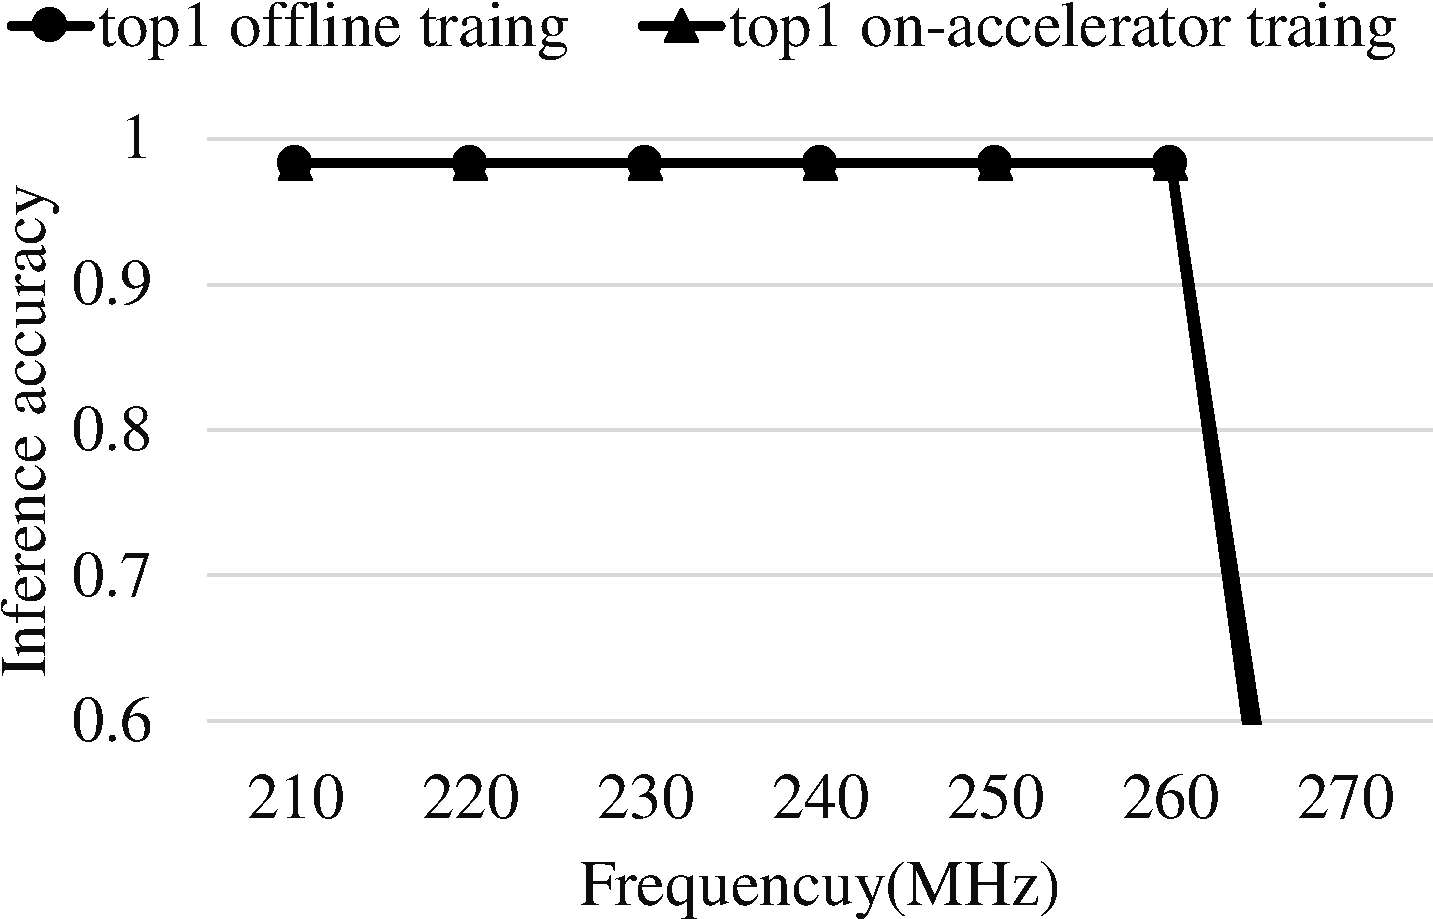
\includegraphics[width=0.65\linewidth]{accuracy_lenet}
	}
	\qquad
	\subfloat[AlexNet]{
                \label{fig:alexnet_accuracy}
                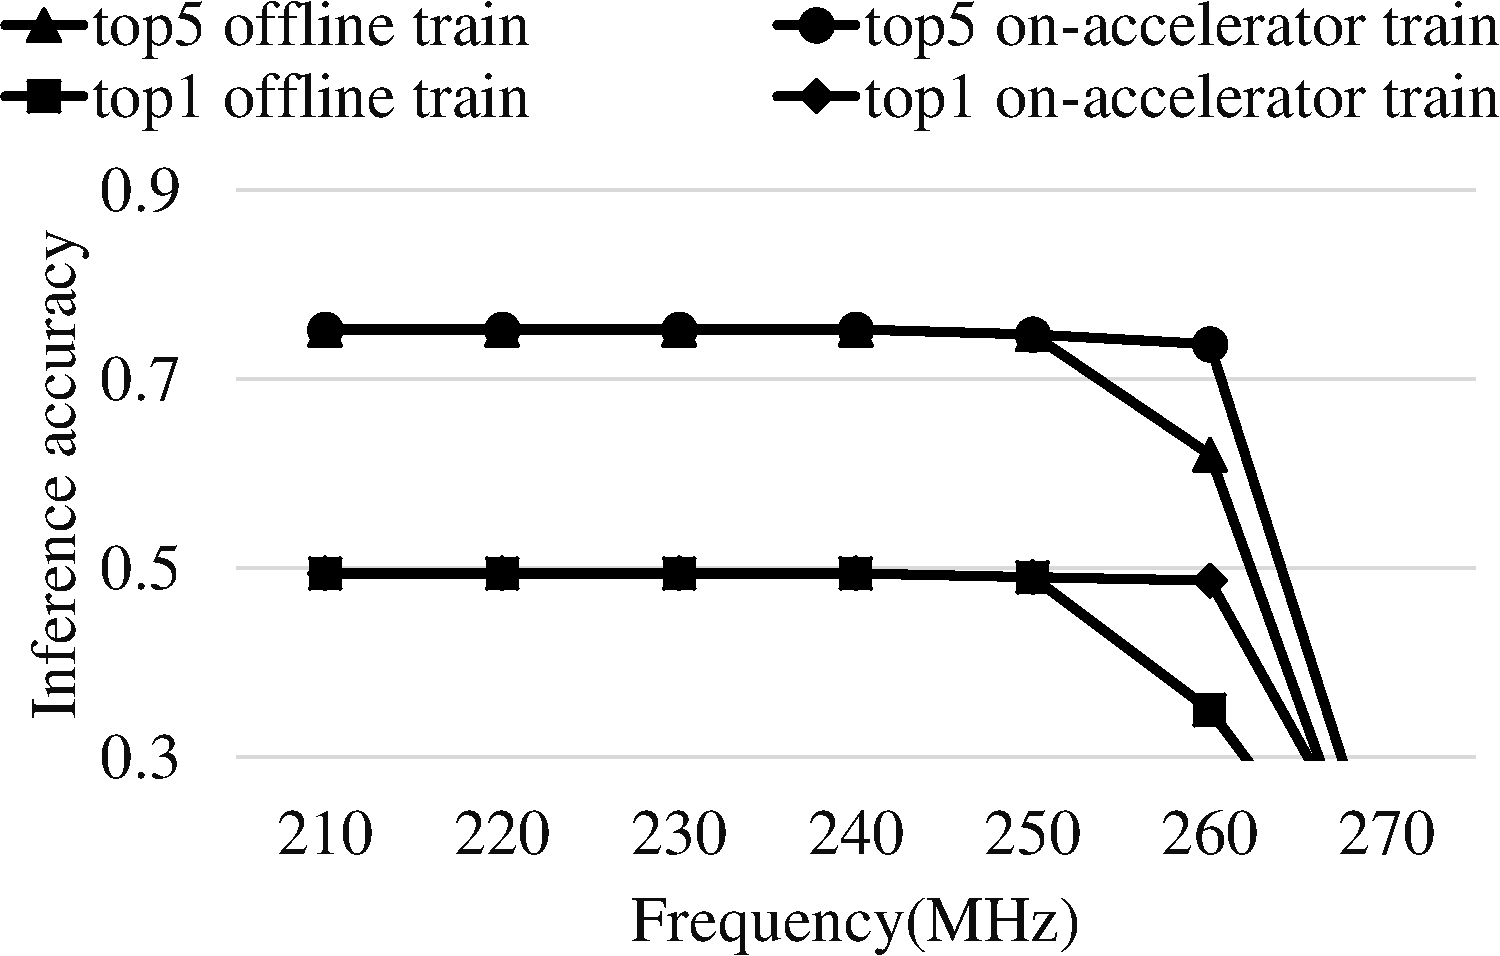
\includegraphics[width=0.65\linewidth]{accuracy_alexnet}
        }
	\qquad
	\subfloat[VGG-16]{
                \label{fig:vgg16_accuracy}
                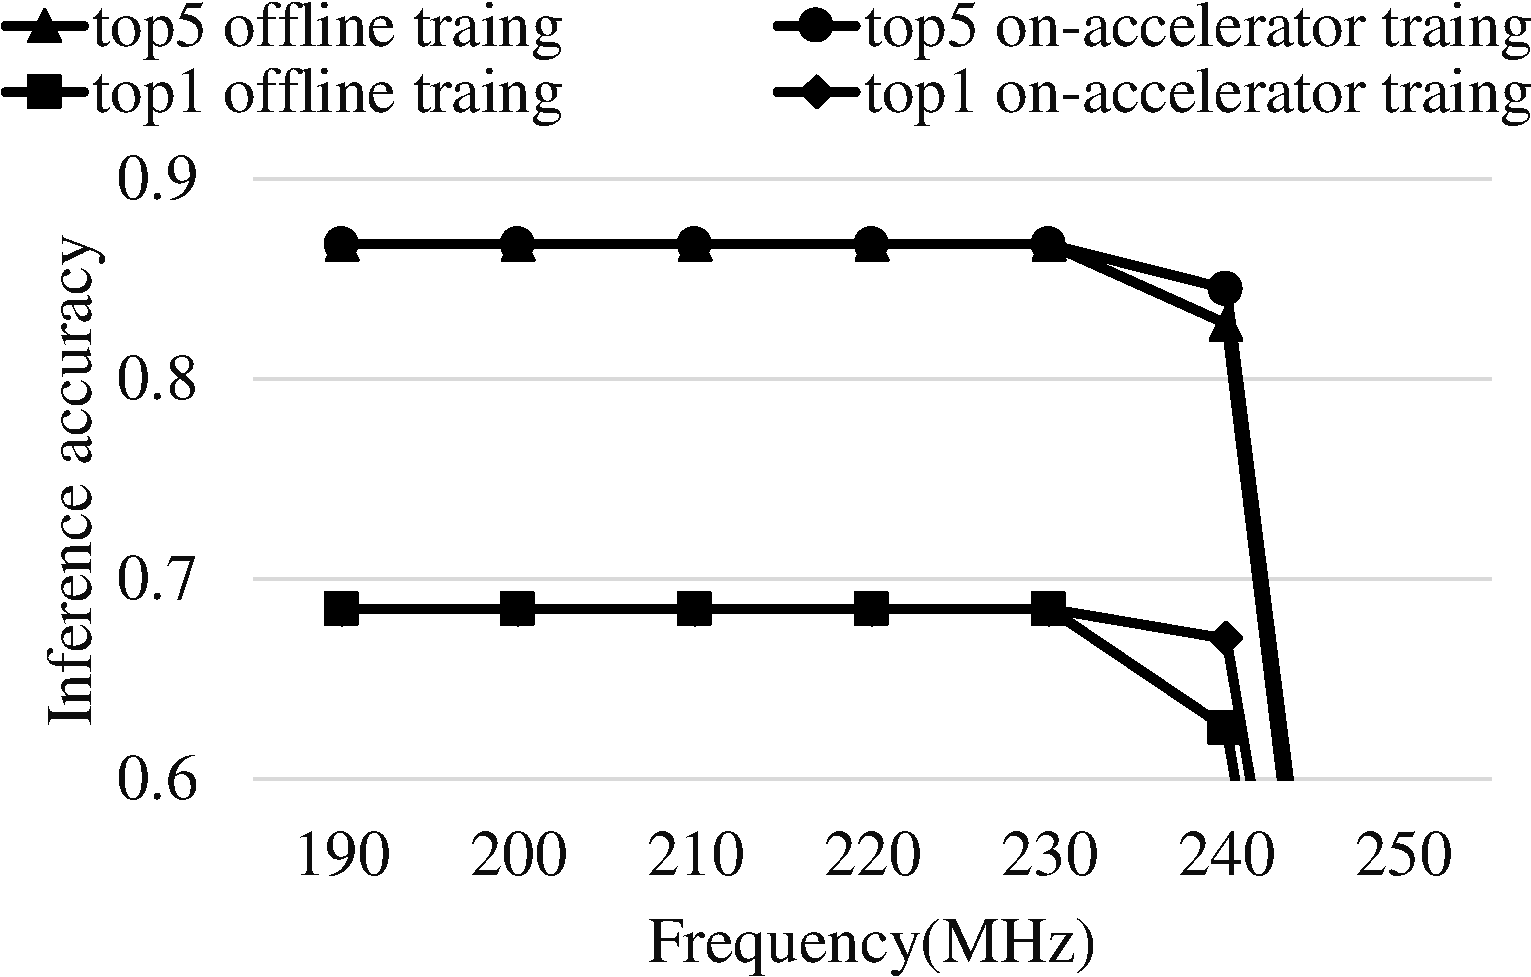
\includegraphics[width=0.65\linewidth]{accuracy_vgg16}
        }
        \qquad
	\subfloat[VGG-19]{
                \label{fig:vgg19_accuracy}
                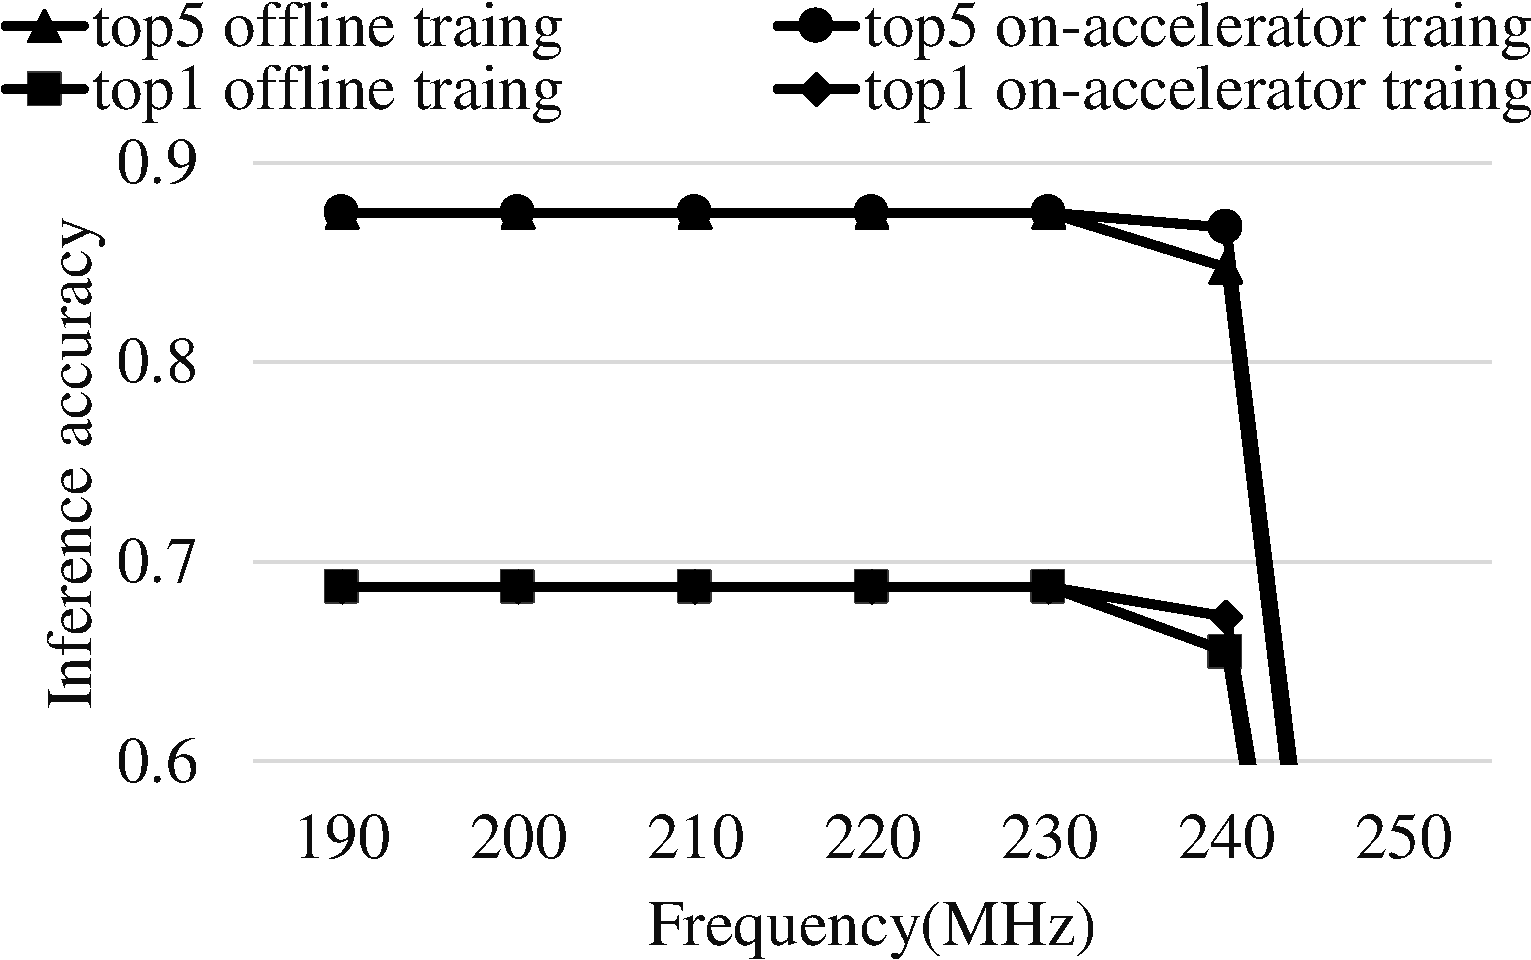
\includegraphics[width=0.65\linewidth]{accuracy_vgg19}
        }
	\caption{The prediction accuracy of the benchmark neural networks on accelerators with different overclocking}
        \label{fig:overclock-accuracy}
		\vspace{-1em}
\end{figure}

We further evaluate the normalized performance over the original CNN accelerators.
As given in Fig \ref{fig:relative_time_overclock}, the performance with the extreme accelerator 
overclocking achieves 1.25X speedup on average compared to the baseline design. 
We use EDP as the energy efficiency metric and compare the 
different overclocking configurations as exhibited in Fig \ref{fig:relative_energy_overclock}.
According to the figure, overclocking on FPGA based CNN 
accelerators achieves more significant energy efficiency improvement when 
compared to the performance improvement. A key reason is that 
the power consumption does not scale much with the clock frequency due to the 
relatively higher background power consumption. On the contrast, 
the performance which contributes more to the EDP metric scales 
much better. 

\begin{figure}
        \center{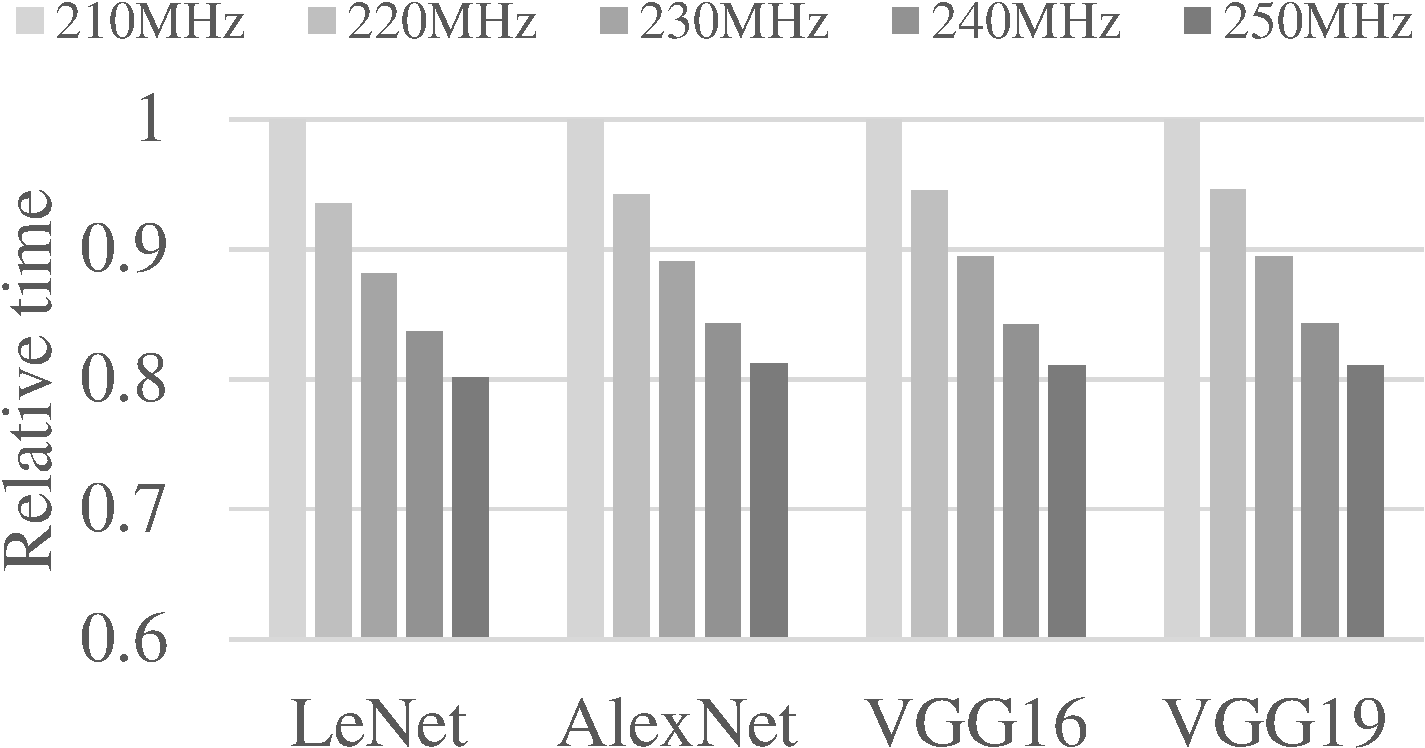
\includegraphics[width=0.65\linewidth]{relative_time_overclock}}
    \caption{Normalized performance of neural networks executed on CNN accelerators with different overclocking.}
\label{fig:relative_time_overclock}
\vspace{-1em}
\end{figure}

\begin{figure}
        \center{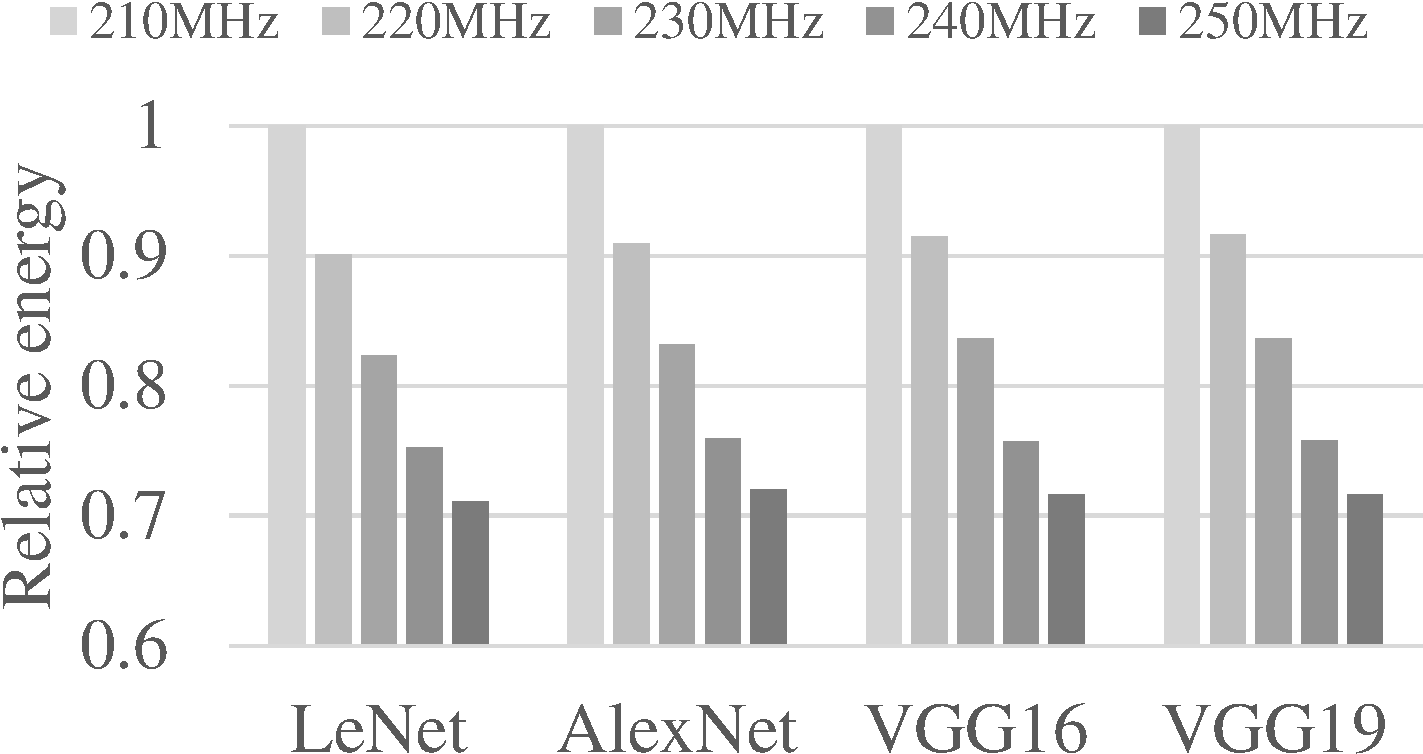
\includegraphics[width=0.65\linewidth]{relative_energy_overclock}}
    \caption{Normalized EDP of neural networks executed on CNN accelerators with different overclocking.}
\label{fig:relative_energy_overclock}
\vspace{-1em}
\end{figure}

In order to quantize the exact computing errors caused by overclocking, we 
particularly analyze the last layer output of the neural networks which 
is typically a vector. We compare it with the output without overclocking.
And we use the percentage of changed output data and the Euclidean distance 
of the output vectors to characterize the difference. 
The comparison is presented in Table \ref{tab:fr_ed}. It can be observed that 
computing errors can be completely hidden by the neural networks when the clock 
frequency is less than 240 MHz in the experiment. Moreover, the small Euclidean indicates that 
the computing error amplitude is relatively small though the percentage of 
the affected results is high when the clock is higher than 240 MHz.

\begin{table}
        \centering
        \vspace{-0.3em}
        \caption{Fault rate and Euclidean distance on the last output layer of the neural network}
        \label{tab:fr_ed}
        \vspace{-0.3em}
        \begin{tabular}{c|cccccc}
                \toprule
                Frequency(MHz) & 210 & 220 & 230 & 240 & 250 & 260 \\
                \midrule
                Euclidean distance & 0 & 0 & 0 & 0 & 35.2 & 104.8 \\
		\midrule
                Fault rate(\%) & 0 & 0 & 0 & 0 & 56.6 & 72.1 \\
                \bottomrule
        \end{tabular}
        \vspace{-1em}
\end{table}

\subsection{Optimization trade-offs}
As discussed in this paper, the timing error can be affected by many factors and it may change 
at runtime. There is no guarantee that the behavior of the CNN accelerator can keep stable even 
overclocking is just slightly higher than the original clock. We use the accelerator overclocked at the 
tipping point to perform the neural network computing. Then we keep measuring its 
prediction accuracy. As shown in Fig \ref{fig:stability}, we find that the accuracy is rather stable.
Although we still can not ensure the stability of the overclocked CNN accelerator, we can 
be sure that the probability of the severe errors such as accelerator hangup or considerable 
accuracy loss is rather low. As we did not observe the cases after processing 100000 pictures, 
we assume the probability of an severe error when processing an input picture is lower than 1/100000.

\begin{figure}
	\center{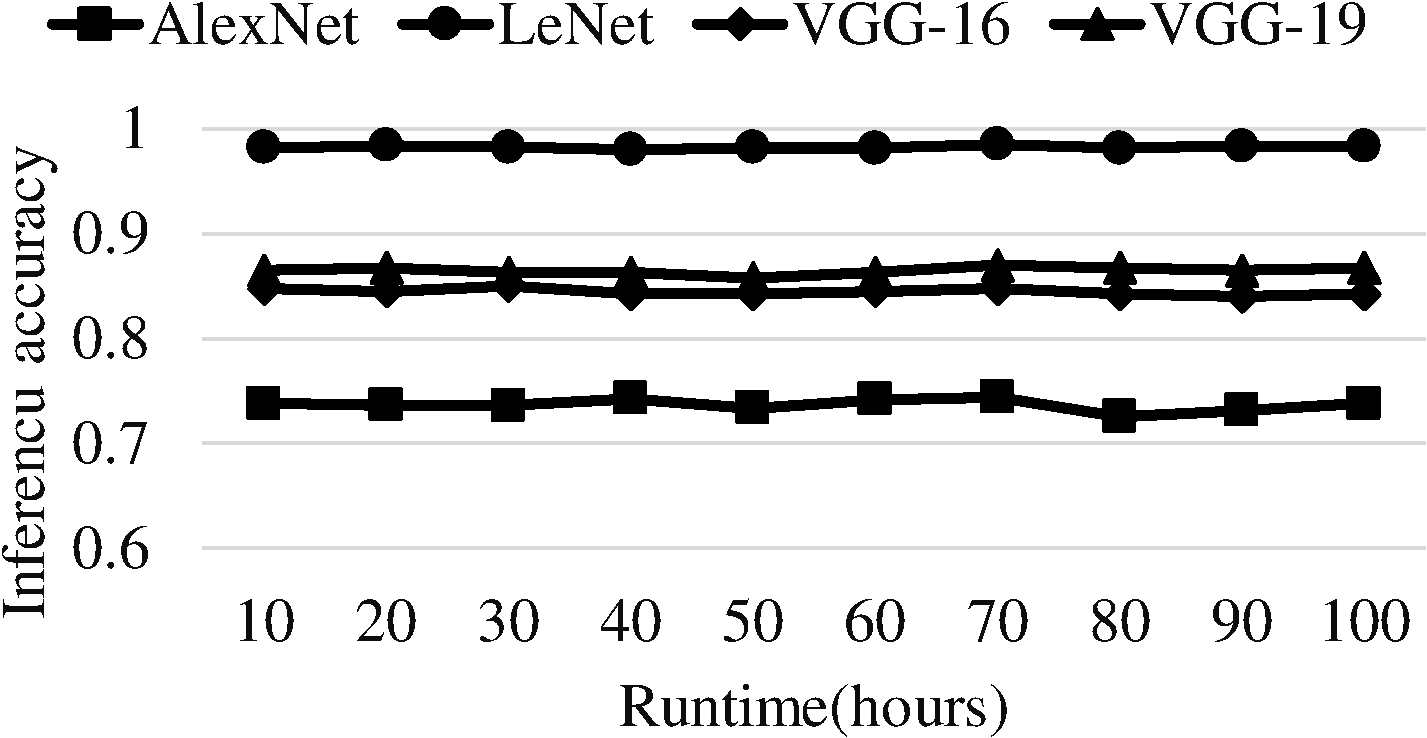
\includegraphics[width=0.65\linewidth]{stability}}
    \caption{Overclocking stability analysis}
\label{fig:stability}
\vspace{-1em}
\end{figure}


With the severe errors, we need to invoke the checkpoint-based error recovery strategy. 
However, this strategy incurs cost including error detection and error recovery. 
We evaluate the overhead of the checkpoint-based strategy. 
A few parameters are critical to the overhead. One of them is the block size, which 
decides the granularity of checkpoint. One of them is the critical 
fault rate. It refers to the probability that CNN accelerator got severe errors 
when processing a single input figure. Another one is the reference data size.

\begin{figure}
        \center{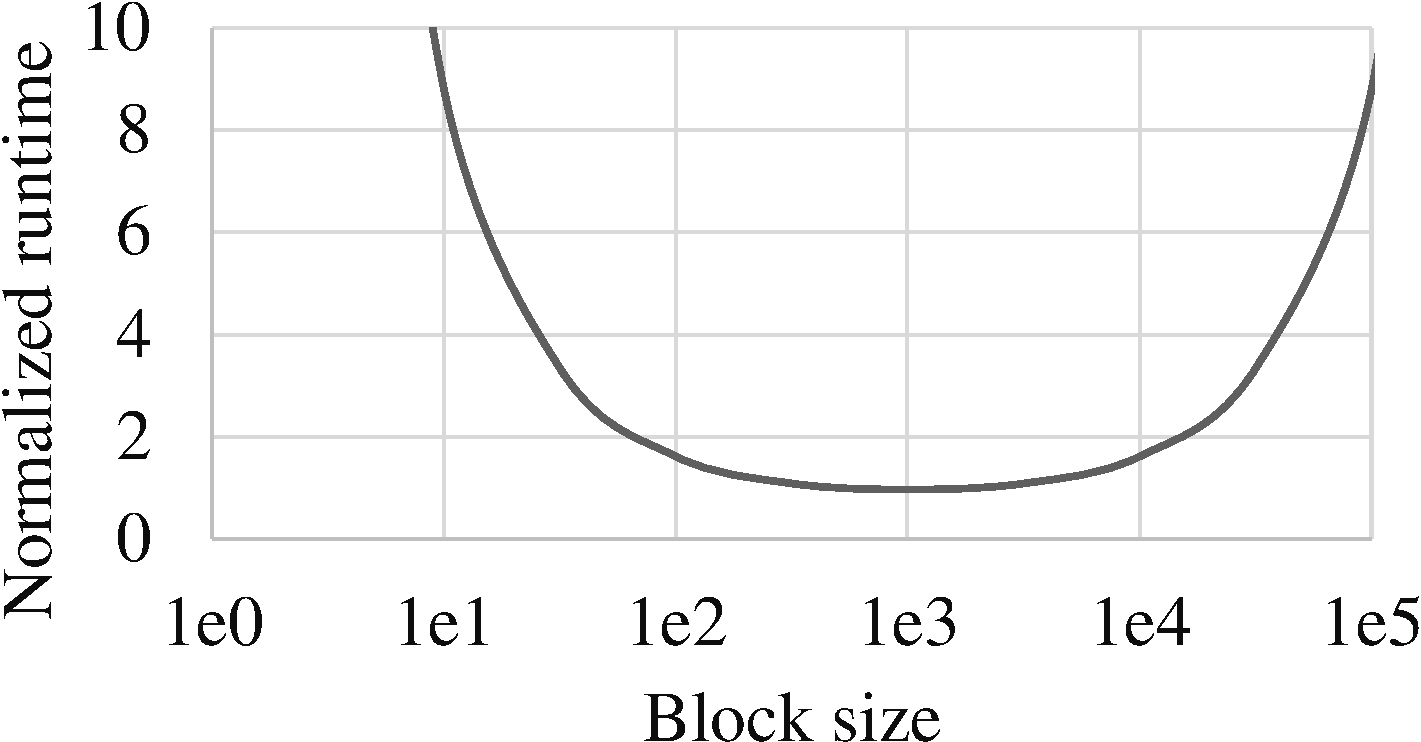
\includegraphics[width=0.65\linewidth]{cost_batch}}
    \caption{The relative overclocking runtime with different block size.}
\label{fig:cost_block}
\vspace{-1em}
\end{figure}

\begin{figure}
	\center{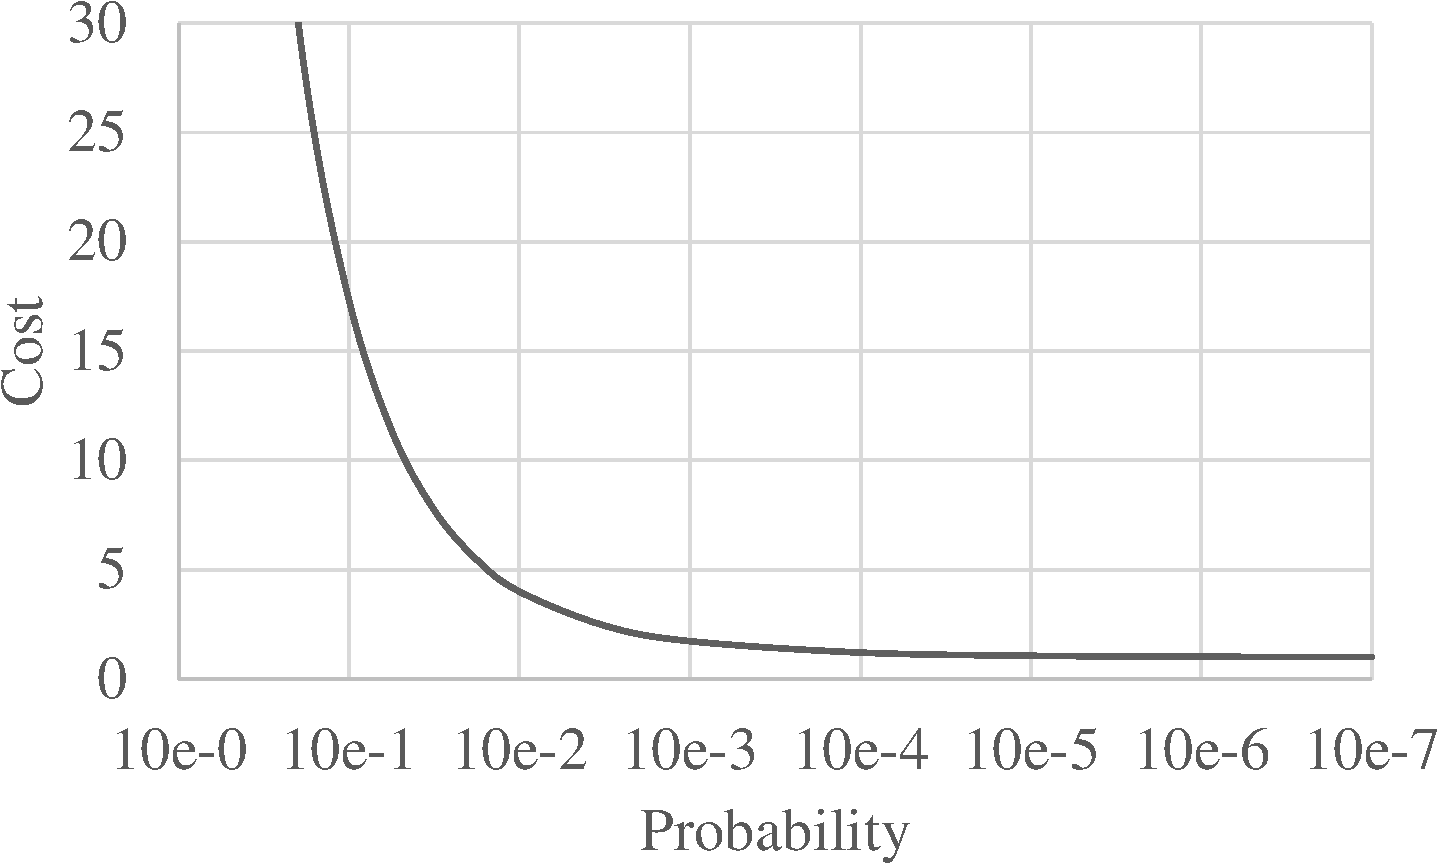
\includegraphics[width=0.65\linewidth]{cost_probability}}
    \caption{The relative overclocking runtime with different fault rate.}
\label{fig:cost_probability}
\vspace{-1em}
\end{figure}


Suppose reference data size is 100 and fault rate under 250 MHz is 1E-5. The relative runtime 
of overclocking over the normal design without overclocking is shown 
in Fig \ref{fig:cost_block}. When the block size is too big, the roll back cost will be 
too large and incurs additional runtime. When the block size is too small, the inserted 
reference data becomes non-trivial and the overall runtime also gets deteoriated. There is 
an optimal block size given specified fault rate and reference data size.
We also analyze the trend of the relative runtime under different fault rate.
As shown in Fig \ref{fig:cost_probability}, the relative runtime increases slightly at 
lower relative fault rate range but grows rapidly when the fault rate is larger than 1E-5.


